\documentclass[12pt]{article}
\usepackage{latexsym,amssymb,amsmath} % for \Box, \mathbb, split, etc.
% \usepackage[]{showkeys} % shows label names
\usepackage{cite} % sorts citation numbers appropriately
\usepackage{path}
\usepackage{url}
\usepackage{verbatim}
\usepackage[pdftex]{graphicx}

% horizontal margins: 1.0 + 6.5 + 1.0 = 8.5
\setlength{\oddsidemargin}{0.0in}
\setlength{\textwidth}{6.5in}
% vertical margins: 1.0 + 9.0 + 1.0 = 11.0
\setlength{\topmargin}{0.0in}
\setlength{\headheight}{12pt}
\setlength{\headsep}{13pt}
\setlength{\textheight}{625pt}
\setlength{\footskip}{24pt}

\renewcommand{\textfraction}{0.10}
\renewcommand{\topfraction}{0.85}
\renewcommand{\bottomfraction}{0.85}
\renewcommand{\floatpagefraction}{0.90}

\makeatletter
\setlength{\arraycolsep}{2\p@} % make spaces around "=" in eqnarray smaller
\makeatother

% change equation, table, figure numbers to be counted inside a section:
\numberwithin{equation}{section}
\numberwithin{table}{section}
\numberwithin{figure}{section}

% begin of personal macros
\newcommand{\half}{{\textstyle \frac{1}{2}}}
\newcommand{\eps}{\varepsilon}
\newcommand{\myth}{\vartheta}
\newcommand{\myphi}{\varphi}

\newcommand{\IN}{\mathbb{N}}
\newcommand{\IZ}{\mathbb{Z}}
\newcommand{\IQ}{\mathbb{Q}}
\newcommand{\IR}{\mathbb{R}}
\newcommand{\IC}{\mathbb{C}}
\newcommand{\Real}[1]{\mathrm{Re}\left({#1}\right)}
\newcommand{\Imag}[1]{\mathrm{Im}\left({#1}\right)}

\newcommand{\norm}[2]{\|{#1}\|_{{}_{#2}}}
\newcommand{\abs}[1]{\left|{#1}\right|}
\newcommand{\ip}[2]{\left\langle {#1}, {#2} \right\rangle}
\newcommand{\der}[2]{\frac{\partial {#1}}{\partial {#2}}}
\newcommand{\dder}[2]{\frac{\partial^2 {#1}}{\partial {#2}^2}}
\usepackage{enumitem}
\newcommand{\nn}{\mathbf{n}}
\newcommand{\xx}{\mathbf{x}}
\newcommand{\uu}{\mathbf{u}}
\usepackage{tikz}
\usetikzlibrary{arrows}
\usetikzlibrary{positioning}
\usepackage{titlesec}
\newcommand{\junk}[1]{{}}
\usepackage{sectsty}
\usepackage{xcolor}

\makeatletter
\renewcommand*\env@matrix[1][\arraystretch]{%
	\edef\arraystretch{#1}%
	\hskip -\arraycolsep
	\let\@ifnextchar\new@ifnextchar
	\array{*\c@MaxMatrixCols c}}
\makeatother

\makeatletter
\renewcommand*\env@matrix[1][*\c@MaxMatrixCols c]{%
	\hskip -\arraycolsep
	\let\@ifnextchar\new@ifnextchar
	\array{#1}}
\makeatother

\definecolor{darkblue}{rgb}{0,0,0.4}
\usepackage[colorlinks = true,
linkcolor = darkblue,
urlcolor  = darkblue,
citecolor = darkblue,
anchorcolor = darkblue]{hyperref}
% set two lengths for the includegraphics commands used to import the plots:
\newlength{\fwtwo} \setlength{\fwtwo}{0.45\textwidth}
% end of personal macros

\begin{document}
\DeclareGraphicsExtensions{.jpg}

\begin{center}
\textsc{\Large Statistical Pattern Recognition} \\[2pt]
	\textsc{\large Assignment 1}\\
	\vspace{0.5cm}
  Ali Gholami \\[6pt]
  Department of Computer Engineering \& Information Technology\\
  Amirkabir University of Technology  \\[6pt]
  \def\UrlFont{\em}
  \url{http://ceit.aut.ac.ir/~aligholamee}\\
    \href{mailto:aligholamee@aut.ac.ir}{\textit{aligholamee@aut.ac.ir}}
\end{center}

\begin{abstract}
This is an introductory assignment to the world of \textit{Statistics} and \textit{Probability} in the context of \textit{Pattern Recognition}. We'll introduce some key concepts like \textit{Probability Distribution Function, Cumulative Distribution Function, Probability Density Function, Probability Mass Function, Joint Probability Density Function, Joint Cumulative Density Function, Marginal Density} \& more details as the probabilistic point of view. Furthermore, we'll review the concepts of \textit{Expected Value, Variance, Standard Deviation, Covariance \& Correlation of Random Variables(e.g. Random Vectors), Univariate \& Multivariate Gaussian Distribution, Total Probability \& Bayes Theorem, Geometric \& Mahalanobis Distances, Central Limit Theorem, Independence \& Correlation} as the statistics point of view. Also, a principal concept called \textit{Linear Transformation} is discussed. The relationship between these fields is far more important than each separately.
\end{abstract}

\subparagraph{Keywords.} \textit{PDF, PMF, JPDF, JPMF, CDF, JCDF, Covariance Matrix, Correlation Coefficient, Correlation, Variance, Expected Vector, Gaussian Distribution, Marginal Probability, Linear Tranformation, Eigenvector, Eigenvalue, Rank.}

\section{Expectation \& Variance}

A random variable \textit{$X$} has \textit{$E(X) = -4$} and \textit{$E(X^2) = 30$.} Let \textit{$Y = -3X + 7$.} Compute the following.

\begin{enumerate}[label=(\alph*)]
	\item \textit{$V(X)$}
	
	\item \textit{$V(Y)$}
	
	\item \textit{$E((X+5)^2)$}
	
	\item \textit{$E(Y^2)$}
	
\end{enumerate}

\titleformat{\section}
{\normalfont\Large\bfseries}   % The style of the section title
{}                             % a prefix
{0pt}                          % How much space exists between the prefix and the title
{Section \thesection:\quad}    % How the section is represented

\subsection*{Solution}

The main equation to calculate the \textit{Variance} of a random variable \textit{X} is given in \ref{eq:1.1}.
\begin{equation}\label{eq:1.1}
	V(X) = E[(X - E[X])^2]
\end{equation}
Expanding the equation \ref{eq:1.1}, we'll have the equation \ref{eq:1.2} using simple calculus.

$$
	V(X) = E[X^2 + E[X]^2 -2XE[X]]
$$
$$
	V(X) = E[X^2] + E[X]^2 - 2E[X]^2
$$
\begin{equation}\label{eq:1.2}
V(X) = E[X^2] - E[X]^2
\end{equation}
\noindent\rule{\textwidth}{.5pt}
(a) The equation \ref{eq:1.2} can be conducted directly to compute the \textit{Variance}. Replacing the values from the problem description we get the following as result.
$$
	V(X) = E[X^2] - E[X]^2 
$$
$$
	V(X) = 30 - 16 = 14
$$
\noindent\rule{\textwidth}{.5pt}
(b) It is important to mention the \textit{Linearity} of \textit{Expectation} operator as formally described in \ref{eq:1.3}.
\begin{equation}\label{eq:1.3}
	E[aX + b] = aE[X] + b
\end{equation}
Using property  \ref{eq:1.3}, we can write the \textit{V(Y)} as

$$
	V(Y) = V(-3X + 7) = E[(-3X + 7)^2] - E[-3X + 7]^2
$$
$$
	V(Y) = E[9X^2 + 49 -42X] - E[-3X + 7]^2
$$
$$
	V(Y) = 9E[X^2] + E[49] - 42E[X] - 9E[X]^2 - E[49]	
$$
$$
	V(Y) = 9*30 + 49 - 42*(-4) - 9*30 - 49
$$
$$
	V(Y) = 168
$$
\noindent\rule{\textwidth}{.5pt}
(c) Expanding the internals of the expectation, we'll get the following.
$$
	E[(X+5)^2] = E[X^2 + 10X + 25]
$$
$$
	E[(X+5)^2] = E[X^2] + 10E[X] + E[25]
$$
$$
	E[(X+5)^2] = 30 + 10*(-4) + 25
$$
$$
	E[(X+5)^2] = 15
$$
\noindent\rule{\textwidth}{.5pt}
(d) Same as above, we'll use 1.2 to get the following.\\
$$
	E[Y^2] = E[(3X + 7)^2]
$$
$$
	E[Y^2] = E[9X^2 + 49 - 42X]
$$
$$
	E[Y^2] = 487
$$

\section{Eigenvector \& Eigenvalue}
(a) Compute eigenvalues and eigenvectors of
$
A = 
	\renewcommand\arraystretch{1}
	\setlength\arraycolsep{6pt}
\begin{bmatrix}
	 4 & 0 & 0 \\
	 0 & 2 & 2 \\
	 0 & 9 & -5 \\
\end{bmatrix}
$
and compare your results with Matlab outputs.
\vspace{.5cm}
\\
(b) A $2*2$ matrix \textit{A} has $\lambda_1 = 2$ and $\lambda_2 = 5$, with corresponding eigenvectors 
$
V_1 = 
	\renewcommand\arraystretch{1}
	\setlength\arraycolsep{6pt}
\begin{bmatrix}
1 & 0
\end{bmatrix}^\mathsf{\textit{T}}
$
and
$
V_2 = 
	\renewcommand\arraystretch{1}
	\setlength\arraycolsep{6pt}
\begin{bmatrix}
1 & 1
\end{bmatrix}^\mathsf{\textit{T}}
$. Find \textit{A}.

\titleformat{\section}
{\normalfont\Large\bfseries}   % The style of the section title
{}                             % a prefix
{0pt}                          % How much space exists between the prefix and the title
{Section \thesection:\quad}    % How the section is represented

\subsection*{Solution}
(a) First of all, we'll find the \textit{eigenvalues} using the \textit{characteristic equation} given in \ref{eq:2.1}.

\begin{equation}\label{eq:2.1}
| A - \lambda I |= 0
\end{equation}
Using this equation, all of the diagonal components of matrix \textit{A} will be decremented by a $\lambda$ term. The determinant of the resulting matrix will be as following.
$$
	A - \lambda I = 
		\renewcommand\arraystretch{1}
		\setlength\arraycolsep{6pt}
	\begin{bmatrix}
	4-\lambda & 0 & 0 \\
	0 & 2-\lambda & 2 \\
	0 & 9 & -5-\lambda \\
	\end{bmatrix}	
$$
$$
| A - \lambda I | = (4-\lambda)(\lambda^2 + 3\lambda - 28)
$$
This will result in the following two roots for the $\lambda$ term.
$$
	\boxed{\lambda_1 = 4} \ \ \ \boxed{\lambda_2 = -7}
$$
These are the \textit{eigenvalues} of the given matrix \textit{A}. We'll continue using the \textit{Gaussian Elimination} technique to compute the \textit{eigenvectors} of matrix \textit{A}. According to the equation \ref{eq:2.2} we are looking for all possible vectors that can be substitute with vector X.
\begin{equation}\label{eq:2.2}
| A - \lambda I |X= 0
\end{equation}
Thus, for each \textit{eigenvalue} determined in the previous computations, we'll find the proper \textit{eigenvector} by converting the equation \ref{eq:2.2} to a \textit{Row Echelon Form} and solving the resulting linear system by \textit{Back Substitution}. Using the computed \textit{eigenvalues}, we'll have \ref{eq:2.3} and \ref{eq:2.4}
\begin{equation}\label{eq:2.3}
	A - 4I = 
		\renewcommand\arraystretch{1}
		\setlength\arraycolsep{6pt}
		\begin{bmatrix}
		0 & 0 & 0 \\
		0 & -2 & 2 \\
		0 & 9 & -9 \\
		\end{bmatrix}
\end{equation}

\begin{equation}\label{eq:2.4}	
	A + 7I = 
		\renewcommand\arraystretch{1}
		\setlength\arraycolsep{6pt}
		\begin{bmatrix}
		11 & 0 & 0 \\
		0 & 9 & 2 \\
		0 & 9 & 2 \\
		\end{bmatrix}
\end{equation}
Now we can find the proper \textit{X} for each \textit{eigenvalue}, using \textit{augmented} version of \ref{eq:2.3} and \ref{eq:2.4}. We'll have \ref{eq:2.5} and \ref{eq:2.6} as result.
\begin{equation}\label{eq:2.5}
	E_1 = (A - 4I \ | \ 0)= 
	\renewcommand\arraystretch{1}
	\setlength\arraycolsep{6pt}
		\begin{bmatrix}[ccc|c]
		0 & 0 & 0 & 0\\	
		0 & -2 & 2 & 0\\
		0 & 9 & -9 & 0\\
		\end{bmatrix}
\end{equation}

\begin{equation}\label{eq:2.6}	
	E_2 = (A + 7I \ | \ 0) = 
	\renewcommand\arraystretch{1}
	\setlength\arraycolsep{6pt}
		\begin{bmatrix}[ccc|c]
		11 & 0 & 0 & 0\\	
		0 & 9 & 2 & 0\\
		0 & 9 & 2 & 0\\
		\end{bmatrix}
\end{equation}
The above matrices will be converted to the \textit{Row Echelon Form} below using \textit{Row Operations.}
$$
	E_1 = 
		\renewcommand\arraystretch{1}
		\setlength\arraycolsep{6pt}
		\begin{bmatrix}[ccc|c]
		0 & 9 & -9 & 0\\	
		0 & -2 & 2 & 0\\
		0 & 9 & -9 & 0\\
		\end{bmatrix}
$$
$$
	E_1 = 
		\renewcommand\arraystretch{1}
		\setlength\arraycolsep{6pt}
		\begin{bmatrix}[ccc|c]
		0 & 9 & -9 & 0\\	
		0 & -2 & 2 & 0\\
		0 & 0 & 0 & 0\\
		\end{bmatrix}
$$
$$
	E_1 = 
	\renewcommand\arraystretch{1}
	\setlength\arraycolsep{6pt}
	\begin{bmatrix}[ccc|c]
	0 & 1 & -1 & 0\\	
	0 & -2 & 2 & 0\\
	0 & 0 & 0 & 0\\
	\end{bmatrix}
$$
$$
E_1 = 
\renewcommand\arraystretch{1}
\setlength\arraycolsep{6pt}
\begin{bmatrix}[ccc|c]
0 & 1 & -1 & 0\\	
0 & 0 & 0 & 0\\
0 & 0 & 0 & 0\\
\end{bmatrix}
$$
The resulting equation for $E_1$ will be as following.
$$
	(0)(X_1) + (1)(X_2) - (1)(X_3) = 0
$$
Thus, we'll have the following \textit{eigenvector} and \textit{eigenvalue}.
$$
	X = 
		\renewcommand\arraystretch{1}
		\setlength\arraycolsep{6pt}
		\begin{bmatrix}[ccc|c]
		X_1\\	
		X_2\\
		X_3\\
		\end{bmatrix} = \renewcommand\arraystretch{1}
		\setlength\arraycolsep{6pt}
		\begin{bmatrix}[ccc|c]
		0\\	
		X_2\\
		X_2\\
		\end{bmatrix}
$$
$$
	X =  X_2 \renewcommand\arraystretch{1}
	\setlength\arraycolsep{6pt}
	\begin{bmatrix}[ccc|c]
	0\\	
	1\\
	1\\
	\end{bmatrix} , \ \ \lambda = 4
$$
for any real number $X_1\neq0$. Calculating the \textit{eigenvector} using the same procedure, we'll get the following results.
\begin{equation}\label{eq:2.7}	
E_2 = (A + 7I \ | \ 0) = 
\renewcommand\arraystretch{1}
\setlength\arraycolsep{6pt}
\begin{bmatrix}[ccc|c]
11 & 0 & 0 & 0\\	
0 & 9 & 2 & 0\\
0 & 9 & 2 & 0\\
\end{bmatrix}
\end{equation}
Using \textit{Row Operations} we'll have:
$$
E_2 = 
\renewcommand\arraystretch{1}
\setlength\arraycolsep{6pt}
\begin{bmatrix}[ccc|c]
11 & 0 & 0 & 0\\	
0 & 9 & 2 & 0\\
0 & 0 & 0 & 0\\
\end{bmatrix}
$$
Since $E_2$ is in the \textit{Row Echelon Form}, we can infer the equation for $E_2$ as:
$$
(11)(X_1) = 0
$$
$$
(9)(X_2) + 2(X_3) = 0
$$
For the \textit{eigenvector} we'll have:
$$
	X =  X_2 \renewcommand\arraystretch{2}
	\setlength\arraycolsep{10pt}
	\begin{bmatrix}[ccc|c]
	0\\	
	1\\
	\frac{-9}{2}\\
	\end{bmatrix} , \ \ \lambda = -7
$$
for any real number $X_2\neq0$.
\subsubsection*{Python Outputs}
\begin{quote}
	\begin{verbatim}
	Eigenvalues:  [-7.  4.  4.]
	Eigenvectors:  [
	[ 0.          0.          1.        ]
	[ 0.21693046 -0.70710678  0.        ]
	[-0.97618706 -0.70710678  0.        ]
	]
	\end{verbatim}
\end{quote}

\subsubsection*{Comparing Results}
The outputs from \textit{linalg.eig} function of \textit{numpy} library depicts that the \textit{eigenvalues} for this matrix are $-7$ and $4$. The eigenvector has been calculated for an specific $X_1$ and $X_2$. In this case we can obtained the outputs by replacing $X_2 = -0.70710$, $X_2 = 1$ and $X_2=0.2169$. Note that having $\lambda = 4$ gives us $y=z$ also which means that we can write its \textit{eigenvector} form like so.
$$
X =  X_2 \renewcommand\arraystretch{1}
\setlength\arraycolsep{6pt}
\begin{bmatrix}[ccc|c]
1\\	
0\\
0\\
\end{bmatrix} , \ \ \lambda = 4
$$

\noindent\rule{\textwidth}{.5pt}
(b) Since \textit{A} is a $2*2$ matrix, we have:
$$
	A = 
	\renewcommand\arraystretch{1}
	\setlength\arraycolsep{6pt}
	\begin{bmatrix}
	a & b\\	
	c & d\\
	\end{bmatrix}
$$
Given \textit{eigenvectors} and \textit{eigenvalues} in the problem description, we can conduct the \textit{Characteristic Equation} presented in \ref{eq:2.2} and get the following results.
$$
(A - 2 I)X = 
\renewcommand\arraystretch{1}
\setlength\arraycolsep{6pt}
\begin{bmatrix}
a-2 & b\\	
c & d-2\\
\end{bmatrix}
\begin{bmatrix}
1\\
0 \\
\end{bmatrix} = \begin{bmatrix}
0\\
0 \\
\end{bmatrix}
$$
$$
(A - 5 I)X = 
\renewcommand\arraystretch{1}
\setlength\arraycolsep{6pt}
\begin{bmatrix}
a-5 & b\\	
c & d-5\\
\end{bmatrix}
\begin{bmatrix}
1\\
1 \\
\end{bmatrix} = \begin{bmatrix}
0\\
0 \\
\end{bmatrix}
$$
Simply solving these equations will give us the following results.
$$
	\boxed{a = 2}
	\ \ \
	\boxed{b = 3}
	\ \ \
	\boxed{c = 0}
	\ \ \
	\boxed{d = 5}
$$
Finally, we'll rewrite the matrix \textit{A} replacing the new parameters in it.
$$
A = 
\renewcommand\arraystretch{1}
\setlength\arraycolsep{6pt}
\begin{bmatrix}
2 & 3\\	
0 & 5\\
\end{bmatrix}
$$
\newpage
\section{Probability Density Function}
Let
\renewcommand\arraystretch{1.2}
\setlength\arraycolsep{10pt}
\[f(x, y) = \left\{
\begin{array}{lr}
c(x + y^2) &  if \ \ 0 < x < 1\ ;\ 0 < y < 1\\
0 &  elsewhere.
\end{array}
\right.
\]
Find each of the following.

\begin{enumerate}[label=(\alph*)]
	\item \textit{$c$}
	
	\item \textit{$f_X (x)$}
	
	\item \textit{$f_{X|Y} (y)$}
	
	\item Are \textit{X} and \textit{Y} independent?
	
	\item What is the probability $Pr(X<\frac{1}{2}  | Y = \frac{1}{2})
	$?
	 
\end{enumerate}

\subsection*{Solution}
(a) The \textit{Joint Probability Distribution} is given above. It is obvious that the total probability is always equal to 1; Hence we can integrate over the variables in the \textit{JPDF} and that will give us the \textit{Total Probability} which is equal to \textit{1}.
$$
\int\limits_{0}^{1} \int\limits_{0}^{1}f(x, y)\ \mathrm{d}x \ \mathrm{d}y=1
$$
Replacing the given equation we'll have the following.
$$
\int\limits_{0}^{1} \int\limits_{0}^{1}c(x+ y^2)\ \mathrm{d}x \ \mathrm{d}y=1
$$ 
$$
\int\limits_{0}^{1}(\frac{c}{2} + cy^2) \ \mathrm{d}y=1
$$ 
$$
	\frac{c}{2} + \frac{c}{3} = 1
$$ 
$$
	\boxed{c = \frac{6}{5}}
$$
\noindent\rule{\textwidth}{.5pt}
(b) \textit{Marginal Density} can easily be computed by integrating over the variable of not interest. 
$$
	f_X (x) = \int_{0}^{1} cx + cy^2 \ \mathrm{d}y
$$
$$
	f_X (x) = \int_{0}^{1} \frac{6x}{5} + \frac{6y^2}{5} \ \mathrm{d}y
$$
$$
	\boxed{f_X (x) = \frac{6x+2}{5}}
$$
\noindent\rule{\textwidth}{.5pt}
(c) While having the relation for the \textit{Joint Probability} and the ease of finding \textit{Marginal Density} of each of the variables, we can simply find the conditional probability using the \textit{Bayes} theorem.
\begin{equation}\label{eq:3.1}
	f_{X|Y} (x) = \frac{f(x, y)}{g(y)}  = \frac{joint\ density\ of\ x\ \&\ y}{marginal\ density\ of\ y}
\end{equation}
The $g(y)$ can be found by integrating the \textit{JPDF} over the variable \textit{X}.
$$
g(y) = \int_{0}^{1} \frac{6}{5}(x+y^2)\ \mathrm{d}x
$$
$$
g(y) = \frac{6y^2}{5} + \frac{3}{2}
$$
Finally, the $f_{X|Y} (x)$ will be:
$$
	f_{X|Y} (x) = \frac{\frac{6}{5}(x+y^2)}{\frac{6y^2}{5} + \frac{3}{2}}
$$
\noindent\rule{\textwidth}{.5pt}
(d) In the case the \textit{X} and \textit{Y} are independent, the conditional probability $f_{X|Y} (x)$ is equal to $f_{X} (x)$. In the previous section, we calculated the $f_{X|Y} (x)$ using \textit{Bayes} theorem. We can simply find $f_{X} (x)$ from the \textit{JPDF} by integrating over \textit{Y}. If the results are equal:
$$
	f_{X|Y} (x) = f_{X} (x)
$$
we say that \textit{X} and \textit{Y} are independent.
Computing the integral of \textit{JPDF} over \textit{Y} we get:
$$
	f_X (x) = \frac{6x+2}{5}
$$
So the variables \textit{X} and \textit{Y} are not \textit{independent}.

\noindent\rule{\textwidth}{.5pt}
(e) Given the conditional density introduced in \ref{eq:3.1}, we'll have:
$$
	Pr(X < \frac{1}{2}\ |\ Y = \frac{1}{2}) = \frac{f(X < \frac{1}{2}, Y = \frac{1}{2})}{g(\frac{1}{2})}
$$
$$
	Pr(X < \frac{1}{2}\ |\ Y = \frac{1}{2}) = \frac{\frac{3}{10}}{\frac{36}{20}}
$$
$$
	Pr(X < \frac{1}{2}\ |\ Y = \frac{1}{2}) = \frac{1}{6}
$$

\section{Multivariate Gaussian Distribution}
Recall the multivariate Gaussian for a vector $x\ \epsilon\ R^n$.
\begin{equation}\label{eq:4.1}
	p(x\ |\ \mu, \Sigma) = \frac{1}{(2\pi)^\frac{n}{2}|\Sigma|^\frac{1}{2}} e^{\frac{-1}{2}(x - \mu)^T\Sigma^{-1}(x - \mu)} 
\end{equation}

\begin{enumerate}[label=(\alph*)]
	\item Let $y=v_i^Tx$, where $v_i$ is an eigenvector of $\Sigma$ with an eigenvalue of $\lambda_i$. Find the probability density of $p(Y)$.
	
	\item Let $X$ be a zero mean Gaussian random vector with an isotropic covariance ($\Sigma  = I$). Let $Y = AX + B$. Compute the mean and variance of $Y$.
	
	\item (\textit{Matlab}) Generate 500 random samples from a 2 dimensional Gaussian with an isotropic $\Sigma$ using the \textit{Matlab} command \textit{\textbf{randn}}. Transform the data as above with
	$
	B = 
	\renewcommand\arraystretch{1}
	\setlength\arraycolsep{6pt}
	\begin{bmatrix}
	0.5 \\
	1 \\
	\end{bmatrix}
	$, and $
	A = 
	\renewcommand\arraystretch{1}
	\setlength\arraycolsep{6pt}
	\begin{bmatrix}
	-5 & 5 \\
	1 & 1 \\
	\end{bmatrix}
	$. Plot the original and transformed points.
	
\end{enumerate}


\subsection*{Solution}
(a) The represented map in section a is a \textit{Linear Map}. Applying a \textit{Linear Map} to a random vector \textit{X} with \textit{mean} $\mu_X$ and \textit{covariance matrix} $\Sigma_X$ will give us a new random vector \textit{Y} with the following properties.
\begin{equation}\label{eq:4.2}
	\boxed{\Sigma_Y = v_i \Sigma v_i^T}
\end{equation}
\begin{equation}\label{eq:4.3}
\boxed{\mu_Y = v_i \mu}
\end{equation}
It is important to mention that the result of a \textit{Linear Map} on a random vector \textit{X} with \textit{Gaussian} distribution will result in variable \text{Y} with \textit{Gaussian} distribution; Hence we can simply represent the new density function for the variable \textit{Y} using the \textit{covariance matrix} and \textit{mean} vector given \ref{eq:4.1}, \ref{eq:4.2} and \ref{eq:4.3}.
\begin{equation}\label{eq:4.4}
p(y\ |\ \mu_Y, \Sigma_Y) = \frac{1}{(2\pi)^\frac{n}{2}|\Sigma_Y|^\frac{1}{2}} e^{\frac{-1}{2}(y - \mu_Y)^T\Sigma_Y^{-1}(y - \mu_Y)} 
\end{equation}
Thus we will have the following probability distribution for random vector \textit{Y}.
$$
p(y\ |\ \mu, \Sigma) = \frac{1}{(2\pi)^\frac{n}{2}|v_i \Sigma v_i^T|^\frac{1}{2}} e^{\frac{-1}{2}(y - v_i \mu)^T(v_i \Sigma v_i^T)^{-1}(y - v_i \mu)}
$$
\textsc{Side note: The eigenvector of a covariance matrix is equal to principal component. The eigenvector with the largest eigenvalue is along which the dataset has the maximum variance. Out interest is to maximize the variance of data in the new dimensional space after applying the linear map.}

\noindent\rule{\textwidth}{.5pt}
(b) A formal representation of the problem description is given below.
$$
	X \sim \mathcal{N}(\mu_X, \ \Sigma_X) = \mathcal{N}(0, \ I)
$$
Note that the isotropic covariance will look like $C=\lambda I$ which in this special case $\lambda = 1$. Applying the linear map $y = Ax + B$ on $X$ will have the following effect on the \textit{mean} and \textit{covariance matrix}.
$$
	Y \sim \mathcal{N}(A\mu_X + B, \ v_i \Sigma_X v_i^T)
$$
$$
	Y \sim \mathcal{N}(B, I)
$$
The new \textit{mean} will be equal to \textit{B} and the new \textit{covariance matrix} will be equal to \textit{I} because:
$$
	Cov(Y) = Cov(AX + B) = A\ \Sigma \ A^T = A\ I\ A^T = A\ A^T\ I = I
$$
\noindent\rule{\textwidth}{.5pt}
(c) The output of the \textit{Axes3D} of \textit{Matplotlib} is given below.
\begin{figure}[!h]\centering
	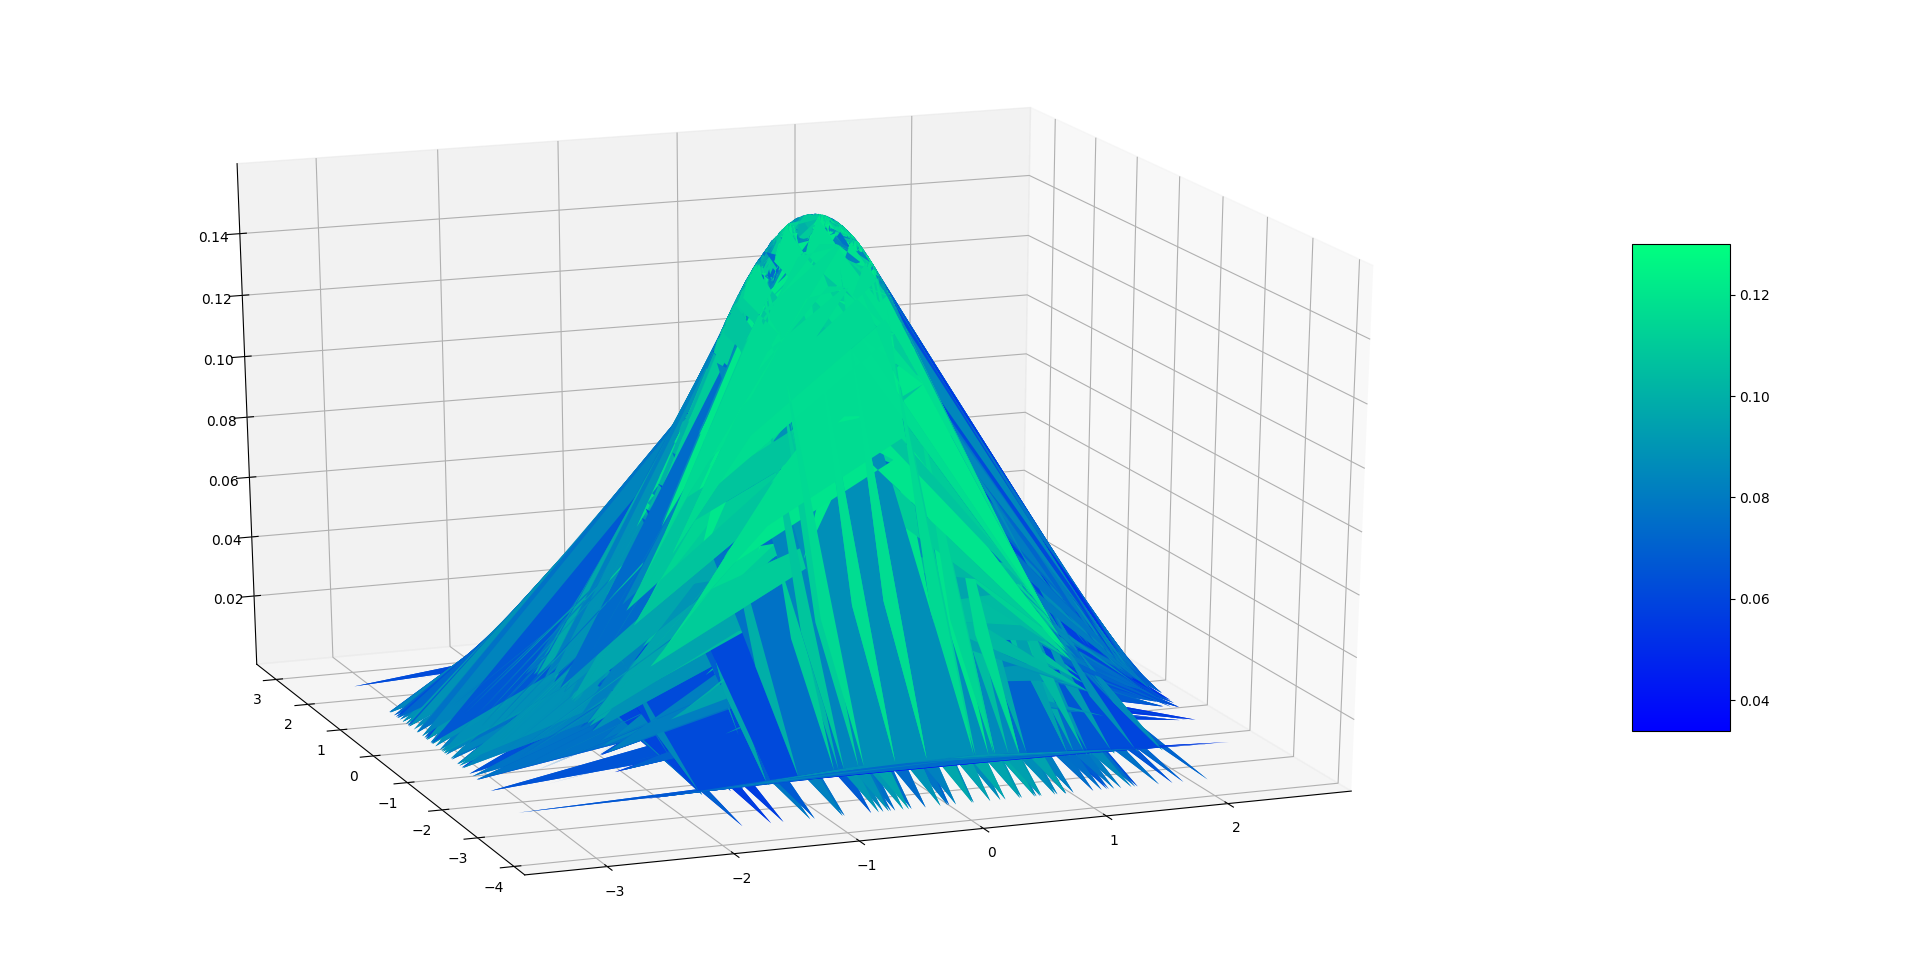
\includegraphics[width=0.45\textwidth]{multivariate_normal.png}
	\caption{3D Plot of a 2D Gaussian distribution with zero mean and isotropic covariance.}
	\label{figsolplot}
\end{figure}
\begin{figure}[!h]\centering
	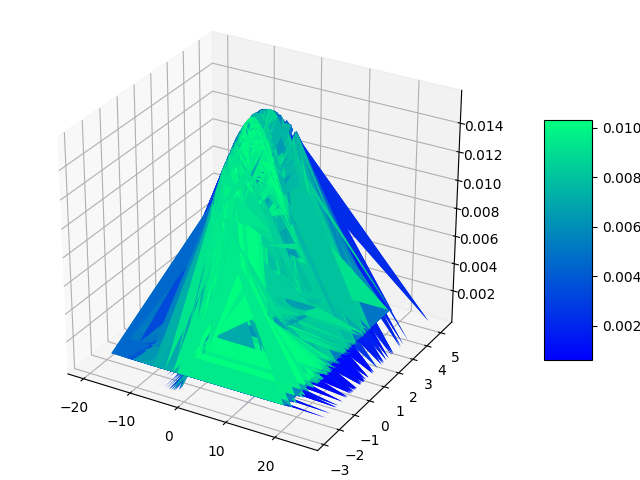
\includegraphics[width=0.45\textwidth]{multivariate_normal_transformed.png}
	\caption{Gaussian distribution after a linear map.}
	\label{figsolplot}
\end{figure}
\newpage

\section{Correlation of Random Variables}
Given $X_1,\ X_2,\ X_3,\ X_4$ as \textit{uncorrelated} random variables each having \textit{mean} 0 and \textit{variance} 1, compute the correlations of:\\
\begin{enumerate}[label=(\alph*)]
	\item $X_1 + X_2$ and $X_2 + X_3$
	
	\item $X_1 + X_2$ and $X_3 + X_4$
\end{enumerate}

\subsection*{Solution}
Before getting into the details of answer, let's talk a bit about the \textit{covariance} and \textit{correlation} terms. They both represent the degree to which two random variables or sets of random variables tend deviate from their expected values. According to the \textit{Wikipedia}, the \textit{covariance} and \textit{correlation} of two random variables $X$ and $Y$ is computed using \ref{eq:5.1} and \ref{eq:5.2} respectively.

\begin{equation}\label{eq:5.1}
	\sigma_{XY} = E[(X-\mu_X)(Y-\mu_Y)]
\end{equation}
\begin{equation}\label{eq:5.2}
	\rho_{XY} = \frac{E[(X-\mu_X)(Y-\mu_Y)]}{\sigma_X\sigma_Y}
\end{equation}
The difference between \textit{covariance} and \textit{correlation} is clear. \textit{correlation} is a \textit{dimensionless} measure and \textit{covariance} is in \textit{units}. Keeping this in mind, we can safely keep moving through the calculation of (a) and (b).\\
(a) Using the covariance equation for two random variables which is given in \ref{eq:5.3} we'
ll get the following.
\begin{equation}\label{eq:5.3}
Cov(A,\ B) = E[AB] - E[A]E[B]
\end{equation}
$$
	Cov(A,\ B) = E[X_1X_2 + X_1X_3 + X_2^2 + X_2X_3] - E[X_1 + X_2]E[X_2 + X_3]
$$
$$
Cov(A,\ B) = E[X_1X_2] + E[X_1X_3] + E[X_2^2] + E[X_2X_3]
$$
$$
\hspace{4.5cm}- E[X_1]E[X_2] - E[X_1]E[X_3] - E[X_2]^2 - E[X_2]E[X_3]
$$
Since the variables are \textit{uncorrelated} pairwise, we have:
$$
	Cov(X_1, X_2) = 0
$$
$$
Cov(X_1, X_3) = 0
$$
$$
Cov(X_1, X_4) = 0
$$
$$
Cov(X_2, X_3) = 0
$$
$$
Cov(X_2, X_4) = 0
$$
$$
Cov(X_3, X_4) = 0
$$
Therefore:
$$
E[X_1X_2] = E[X_1]E[X_2]
$$
$$
E[X_1X_3] = E[X_1]E[X_3]
$$
$$
E[X_2X_3] = E[X_2]E[X_3]
$$
Finally, the results for the $Cov(A,\ B)$ will be:
$$
	Cov(A,\ B) = E[X_2^2] - E[X_2]^2
$$
which is the \textit{variance} of $X_2$ according to the \ref{eq:1.2} and the value of that is equal to 1 according to the problem description. Thus, we'll have the following result for the correlation of $A=X_1+X_2$ and $B=X_2+X_3$.
$$
\boxed{\rho_{AB} =	1}
$$
Which represents that \textit{A} and \textit{B} have a \textit{perfect positive} relationship; when one variable moves higher or lower, the other variable moves in the same direction with the same magnitude.

\noindent\rule{\textwidth}{.5pt}
(b) Using the same terminology as previous section, we'll have the following computations to find the correlation of $A = X_1 + X_2$ and $B = X_3 + X_4$.
$$
Cov(A,\ B) = E[X_1X_3 + X_1X_4 + X_2X_3 + X_2X_4] - E[X_1 + X_2]E[X_3 + X_4]
$$
$$
Cov(A,\ B) = E[X_1X_3] + E[X_1X_4] + E[X_2X_3] + E[X_2X_4]
$$
$$
\hspace{4.5cm}- E[X_1]E[X_3] - E[X_1]E[X_4] - E[X_2]E[X_3] - E[X_2]E[X_4]
$$
$$
	Cov(A,\ B) = 0
$$
$$
\boxed{\rho_{AB} =	0}
$$

\section{Independence \& Expectation}
If $X$ and $Y$ are \textit{independent} and \textit{identically distributed} with \textit{mean} $\lambda$ and \textit{variance} $\sigma^2$, find $E[(X-Y)^2]$.

\subsection*{Solution}
We have the following information about $X$ and $Y$ random variables:\\
$$
	E[X] = \lambda
$$
$$
	E[Y] = \lambda
$$
$$
	V[X] = \sigma^2
$$
$$
	V[Y] = \sigma^2
$$
Expanding the given equation for the $X$ and $Y$ we get:
$$
	E[(X-Y)^2] = E[X^2] + E[Y^2] - 2E[X]E[Y]
$$	
\begin{equation}\label{eq:6.1}
E[(X-Y)^2] = E[X^2] + E[Y^2] - 2\lambda^2
\end{equation}
Using the equation \ref{eq:1.2} we can simply find $E[X^2]$ and $E[Y^2]$:
$$
	E[X^2] = \sigma^2 + \lambda^2
$$
$$
	E[Y^2] = \sigma^2 + \lambda^2
$$
Replacing with materials in equation \ref{eq:6.1} we'll get:
$$
	\boxed{E[(X-Y)^2] = 2(\sigma^2 + \lambda^2)- 2\lambda^2 = 2\sigma^2}	
$$
\section{Marginal \& Conditional Density}
Let $p(X)$ be $\mathcal{N}(M, \Sigma)$ with
$$
	X = \begin{bmatrix}
	x_1\\	
	x_2\\
	\end{bmatrix},\ \ \ 
	M = \begin{bmatrix}
	m_1\\	
	m_2\\
	\end{bmatrix}\ and\ \ 
	\Sigma = \begin{bmatrix}
	\sigma_1^2 & \rho\sigma_1\sigma_2\\	
	\rho\sigma_1\sigma_2\ & \sigma_2^2\\
	\end{bmatrix}
$$
Show that:
\begin{enumerate}[label=(\alph*)]
	\item $p(x_1) \sim \mathcal{N}_{x_1}(m_1,\ \sigma_1^2)\ \ $  (\textit{a marginal density})
	\item $p(x_1\ |\ x_2) \sim \mathcal{N}_{x_1}(m_1 + \frac{\rho\sigma_1(x_2 - m_2)}{\sigma_2},\ \sigma_1^2(1-\rho^2))\ \ $ (\textit{a conditional density})
\end{enumerate}

\subsection*{Solution}
Since we'll need some \textit{inverse matrix} computations, we need to review two theorems. The first theorem is about \textit{inverse of a partitioned symmetric matrix} which divides every square matrix into 4 blocks. Correspondingly, the inverse matrix will be divided into 4 blocks and the inverse of these blocks can be calculated separately.

\subsubsection*{Theorem 1}
Let A = $
	\renewcommand\arraystretch{1}
	\setlength\arraycolsep{6pt}
	\begin{bmatrix}
	A_{11} & A_{12} \\
	A_{12}^T & A_{22}\\
	\end{bmatrix}$,
which demonstrates the division of every square matrix into 4 blocks. The inverse matrix $B=A^{-1}$ can also be divided into four blocks.
$$
	 B = A^{-1} = 
	 \renewcommand\arraystretch{1}
	 \setlength\arraycolsep{6pt}
	 \begin{bmatrix}
	 B_{11} & B_{12} \\
	 B_{12}^T & B_{22}\\
 \end{bmatrix}
$$
Now we can separately compute each of the components of inverse matrix.
$$
	B_{11} = (A_{11} - A_{12}A_{22}^{-1}A_{12}^{T})^{-1} = A_{11}^{-1} + A_{11}^{-1}A_{12}(A_{22} - A_{12}^{T}A_{11}^{-1}A_{12})^{-1}A_{12}^{T}A_{11}^{-1}
$$
$$
B_{22} = (A_{22} - A_{12}^{T}A_{11}^{-1}A_{12})^{-1} = A_{22}^{-1} + A_{22}^{-1}A_{12}^{T}(A_{11} - A_{12}A_{22}^{-1}A_{12}^{T})^{-1}A_{12}A_{22}^{-1}
$$
$$
B_{12} = -A_{22}^{-1}A_{12}^{T}(A_{11}-A_{12}A_{22}^{-1}A_{12}^T)^{-1}
$$
$$
B_{12}^{T} = -A_{11}^{-1}A_{12}(A_{22}-A_{12}^{T}A_{11}^{-1}A_{12})^{-1}
$$

\subsubsection*{Theorem 2}
Let A = $
\renewcommand\arraystretch{1}
\setlength\arraycolsep{6pt}
\begin{bmatrix}
A_{11} & A_{12} \\
A_{21} & A_{22}\\
\end{bmatrix}$, which $A$ is a partitioned symmetric matrix. We can compute the determinant of matrix $A$ using the following formula:
$$
\begin{vmatrix}
A
\end{vmatrix}=
	\renewcommand\arraystretch{1}
	\setlength\arraycolsep{6pt}
	\begin{vmatrix}
	A_{11} & A_{12} \\
	A_{21} & A_{22}\\
	\end{vmatrix} = 
	\begin{vmatrix}
	A_{11}
	\end{vmatrix}\begin{vmatrix}
	A_{22} - A_{12}^TA_{11}^{-1}A_{12}
	\end{vmatrix}=\begin{vmatrix}
	A_{22}
	\end{vmatrix}\begin{vmatrix}
	A_{11} - A_{11}A_{22}^{-1}A_{12}^T
	\end{vmatrix}
$$
Now let's derive the \textit{multivariate Gaussian} for vector $X$. The \textit{joint density} of \textit{X} is:
\begin{equation}\label{eq:7.1}
p(x_1,\ x_2\ |\ \mu, \Sigma) = \frac{1}{(2\pi)^\frac{n}{2}|\Sigma|^\frac{1}{2}} e^{\frac{-1}{2}D(x_1,\ x_2)} 
\end{equation}
Expanding the $D(x_1,\ x_2)$ as a matrix multiplication, we get:
$$
	D(x_1, x_2) = \renewcommand\arraystretch{1}
	\setlength\arraycolsep{6pt}
	\begin{bmatrix}
	x_1 - \mu_1\\
	x_2 - \mu_2\\
	\end{bmatrix}^T
	\renewcommand\arraystretch{1}
	\setlength\arraycolsep{6pt}
	\begin{bmatrix}
	\Sigma_{11} & \Sigma_{12} \\
	\Sigma_{21} & \Sigma_{22}\\
	\end{bmatrix}^{-1}\renewcommand\arraystretch{1}
	\setlength\arraycolsep{6pt}
	\begin{bmatrix}
	x_1 - \mu_1\\
	x_2 - \mu_2\\
	\end{bmatrix}	
$$
The inverse matrix will be displayed with $\Sigma^{ij}$ according to the conventions. Thus, by using \textit{Theorem 1} we get:
$$
	D(x_1,\ x_2) = \renewcommand\arraystretch{1}
	\setlength\arraycolsep{6pt}
	\begin{bmatrix}
	{(x_1 - \mu_1)}^{T}\ 
	{(x_2 - \mu_2)}^{T}\\
	\end{bmatrix}
	\renewcommand\arraystretch{1}
	\setlength\arraycolsep{6pt}
	\begin{bmatrix}
	\Sigma^{11} & \Sigma^{12} \\
	\Sigma^{21} & \Sigma^{22}\\
	\end{bmatrix}\renewcommand\arraystretch{1}
	\setlength\arraycolsep{6pt}
	\begin{bmatrix}
	x_1 - \mu_1\\
	x_2 - \mu_2\\
	\end{bmatrix}	
$$
The result of the multiplication can be shown as following.
$$
	D(x_1,\ x_2) = (x_1 - \mu_1)^{T}\Sigma^{11}(x_1 - \mu_1) + 2(x_1 - \mu_1)^T\Sigma^{12}(x_2- \mu_2) + (x_2-\mu_2)^T\Sigma^{22}(x_2-\mu_2)
$$
We will replace the $\Sigma^{11},\ \Sigma^{12}$ and $\Sigma^{22}$ with the result from \textit{Theorem 2}. 
$$
	D(x_1,\ x_2) = (x_1 - \mu_1)^{T}[\Sigma_{11}^{-1} + \Sigma_{11}^{-1}\Sigma_{12}(\Sigma_{22} - \Sigma_{12}^{T}\Sigma_{11}^{-1}\Sigma_{12})^{-1}\Sigma_{12}^{T}\Sigma_{11}^{-1}](x_1 - \mu_1)
$$
$$
	-2(x_1 - \mu_1)^{T}[\Sigma_{11}^{-1}\Sigma_{12}(\Sigma_{22} - \Sigma_{12}^{T} \Sigma_{11}^{-1}\Sigma_{12})^{-1}](x_2-\mu_2)
$$
$$
	+(x_2 - \mu_2)^{T}[(\Sigma_{22} - \Sigma_{12}^T\Sigma_{11}^{-1}\Sigma_{12})^{-1}](x_2- \mu_2)
$$
Applying multiplication on the first term we get:
$$
D(x_1,\ x_2) = (x_1 - \mu_1)^{T}\Sigma_{11}^{-1}(x_1 - \mu_1)
$$
$$
	+ (x_1 - \mu_1)^{T}[ \Sigma_{11}^{-1}\Sigma_{12}(\Sigma_{22} - \Sigma_{12}^{T}\Sigma_{11}^{-1}\Sigma_{12})^{-1}\Sigma_{12}^{T}\Sigma_{11}^{-1}](x_1 - \mu_1)
$$
$$
-2(x_1 - \mu_1)^{T}[\Sigma_{11}^{-1}\Sigma_{12}(\Sigma_{22} - \Sigma_{12}^{T} \Sigma_{11}^{-1}\Sigma_{12})^{-1}](x_2-\mu_2)
$$
$$
+(x_2 - \mu_2)^{T}[(\Sigma_{22} - \Sigma_{12}^T\Sigma_{11}^{-1}\Sigma_{12})^{-1}](x_2- \mu_2)
$$
Now we conduct another \textit{Theorem} to display the $D(x_1,\ x_2)$ in a more compact form.
\subsubsection*{Theorem 3}
Given symmetric matrix equation $A = A^T$, for any vectors $u$ and $v$ we have:
$$
	u^TAu - 2u^TAv+ v^TAv = (v-u)^TA(v-u)
$$ 
Applying \textit{Theorem 3} on $D(x_1,\ x_2)$:
$$
	D(x_1,\ x_2) = (x_1 - \mu_1)^T\Sigma_{11}^{-1}(x_1 - \mu_1)
$$
$$
	+[(x_2 - \mu_2) - \Sigma_{12}^T\Sigma_{11}^{-1}(x_1 - \mu_1)]^T(\Sigma_{22} - \Sigma_{12}^T\Sigma_{11}^{-1}\Sigma_{12})^{-1}[(x_2 - \mu_2) - \Sigma_{12}^T\Sigma_{11}^{-1}(x_1 - \mu_1)]
$$
Let's define
$$
	\boxed{	A = \Sigma_{22} - \Sigma_{12}^{T}\Sigma_{11}^{-1}\Sigma_{12}}
$$
$$
	\boxed{	b = \mu_2 + \Sigma_{12}^T\Sigma_{11}^{-1}(x_1 - \mu_1)}
$$
and 
$$
	D_{1}(x_1) = (x_1 - \mu_1)^{T}\Sigma_{11}^{-1}(x_1 - \mu_1)
$$
$$
	D_{2}(x_1,\ x_2) = (x_2 - b)^{T}A^{-1}(x_2-b)
$$
Thus we will have
$$
	D(x_1,\ x_2) = D_1(x_1) + D_2(x_1,\ x_2)
$$
Now we can rewrite the joint distribution as 
$$
	p(x_1,\ x_2\ |\ \mu, \Sigma) = \frac{1}{(2\pi)^\frac{n}{2}|\Sigma|^\frac{1}{2}} e^{\frac{-1}{2}D(x_1,\ x_2)}
$$
Now according to the \textit{Theorem 3} we get
$$
	\begin{vmatrix}
		\Sigma
	\end{vmatrix} = \begin{vmatrix}
		\Sigma_{11}
	\end{vmatrix}
	\begin{vmatrix}
		\Sigma_{22} - \Sigma_{12}^T\Sigma_{11}^{-1}\Sigma_{12}
	\end{vmatrix}
$$
Replacing in the joint probability we get
$$
p(x_1,\ x_2\ |\ \mu, \Sigma) = \frac{1}{(2\pi)^\frac{n}{2}|\Sigma_{11}|^\frac{1}{2}|\Sigma_{22} - \Sigma_{12}^T\Sigma_{11}^{-1}\Sigma_{12}|^\frac{1}{2}} e^{\frac{-1}{2}D(x_1,\ x_2)}
$$
Separating $x_1$ and $x_2$ according to the definitions above, we'll have the following result for each of the random variables (\textit{this proof is for the general mode, the question has asked for the simple 2*2 mode.})
$$
	p(x_1,\ x_2\ |\ \mu,\ \Sigma) = \mathcal{N}_{x_1}(\mu_1,\ \Sigma_{11})\mathcal{N}_{x_2}(b,\ A)
$$
which in this special case, we have
$$
X = \begin{bmatrix}
x_1\\	
x_2\\
\end{bmatrix},\ \ \ 
M = \begin{bmatrix}
m_1\\	
m_2\\
\end{bmatrix}\ and\ \ 
\Sigma = \begin{bmatrix}
\sigma_1^2 & \rho\sigma_1\sigma_2\\	
\rho\sigma_1\sigma_2\ & \sigma_2^2\\
\end{bmatrix}
$$
Thus, the \textit{separated distribution} of $x_1$ and $x_2$ will be:
$$
	p(x_1,\ x_2\ |\ \mu,\ \Sigma) = \mathcal{N}_{x_1}(m_1,\ \sigma_{1}^2)\mathcal{N}_{x_2}(b,\ A)
$$
Finally, the \textit{marginal density} of $x_1$ is
$$
	p(x_1) = \int_{}^{}p(x_1,\ x_2)\mathrm{d}x_2 = \frac{1}{2\pi|\sigma_{1}^2|^\frac{1}{2}} e^{\frac{-1}{2}(x_1 - m_1)^T\Sigma^{-1}(x_1 - m_1)}
$$
Thus we get the following \textit{marginal densities} as result.
$$
	p(x_1) \sim \mathcal{N}_{x_1}(m_1,\ \sigma_1^2)\ \
$$
$$
	p(x_2) \sim \mathcal{N}_{x_2}(m_2,\ \sigma_2^2)\ \
$$
For the \textit{conditional density} of $p(x_1\ |\ x_2)$ we will divide the \textit{joint probability} to the forsaken \textit{marginal probability}. Replacing $b$ and $A$ from the problem description we get:
$$
	p(x_1\ |\ x_2) = \frac{p(x_1,\ x_2)}{p(x_2)} = \frac{1}{2\pi|\sigma_{2}^2 - (\rho\sigma_1\sigma_2)^2(\sigma_1)^2|^\frac{1}{2}} e^{\frac{-1}{2}(x_2 - m_2 - (\rho\sigma_1\sigma_2)(\sigma_1)^2)^T\Sigma^{-1}(x_2 - m_2 - (\rho\sigma_1\sigma_2)(\sigma_1)^2)}
$$
Which denotes that
$$
p(x_1\ |\ x_2) \sim \mathcal{N}_{x_1}(m_1 + \frac{\rho\sigma_1(x_2 - m_2)}{\sigma_2},\ \sigma_1^2(1-\rho^2))
$$
\end{document}